\section{Investigation}

\ctt{To do: understands how the investigation should look like. Plot an example to such tree.}
The model goes as follow, at each even iteration we toss a noise, then in each odd iteration we perform a single SWEEP rule iteration. That allows to track over the history of the errors.  

We say that a check $e \in $ Error, if there is a face $f$ that adjoin to $e$ and belongs to the Error. 


\begin{definition}[Investigation]
  For any unsatisfied check $e$ at time $t$, we define $V$ (the set of checks which participated in 'misleading' of $e$), and two sets of edges on $V$, Arrows and Forks via the following algorithm: 


  

\end{definition}
\tikzset{%
  every neuron/.style={
    circle,
    draw,
    %fill=black,
    radius=0.1mm
  },
  neuron missing/.style={
    draw=none,
    scale=2,
    text height=0.25cm,
    execute at begin node=\color{black}$\vdots$
  },
}

  \begin{figure}[h]
    \centering
  \begin{algorithm}[H]
    let $V = \{e\}$, Arrows $= \emptyset$, Forks $= \emptyset$\\
    let $Q \leftarrow $ queue $\{ e \}$\\
    \While{ $Q$ is not empty  }{
      $e^{\prime} \leftarrow $ dequeue $Q$ \\
      \If { $e^{\prime} \notin $ Error }{
        $e_{1},..,e_{l} \leftarrow $ Excuse( $e^{\prime}$ ) \\
        Insert $\{e_{i}, e^{\prime} \}$ to Arrows\\
        Insert $\{e_{i}, e_{j} \}$ to Forks
      }
    }
    %\caption{Investigation}
  \end{algorithm}
\end{figure}
\begin{figure}[h]
      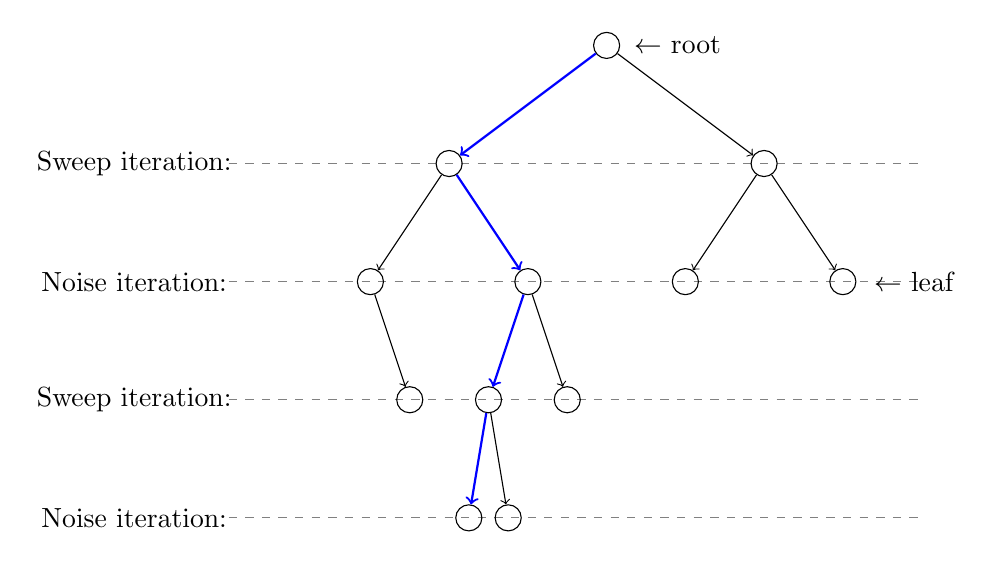
\begin{tikzpicture}[scale=1]%[ultra thick]
  \draw [dashed, draw=gray] (-1.8,-1.5) -- (7,-1.5);
  \draw [dashed, draw=gray] (-1.8,-3) -- (7,-3);
  \draw [dashed, draw=gray] (-1.8,-4.5) -- (7,-4.5);
  \draw [dashed, draw=gray] (-1.8,-6) -- (7,-6);
  \node (SWEEP1) at (-3, -1.5) {Sweep iteration: };
  \node (NOISE1) at (-3, -3) {Noise iteration: };
  \node (SWEEP2) at (-3, -4.5) {Sweep iteration: };
  \node (NOISE2) at (-3, -6) {Noise iteration: };
  \node (root) at (3.9, -0) { $\leftarrow$ root };
  \node (root) at (6.9, -3) { $\leftarrow$ leaf };
  \node [every  neuron ] (v-1) at ( 3 ,-0) { } ;
  \node [every  neuron ] (v-2) at ( 1 ,-1.5) { } ;
  \node [every  neuron ] (v-3) at ( 5 ,-1.5) { } ;
  \node [every  neuron ] (v-4) at ( 0 ,-3) { } ;
  \node [every  neuron ] (v-5) at ( 2 ,-3) { } ;
  \node [every  neuron ] (v-6) at ( 4 ,-3) { } ;
  \node [every  neuron ] (v-7) at ( 6 ,-3) { } ;
  \node [every  neuron ] (v-8) at ( 0.5 ,-4.5) { } ;
  \node [every  neuron ] (v-9) at ( 1.5 ,-4.5) { } ;
  \node [every  neuron ] (v-10) at ( 2.5 ,-4.5) { } ;
  \node [every  neuron ] (v-11) at ( 1.25 ,-6) { } ;
  \node [every  neuron ] (v-12) at ( 1.75 ,-6) { } ;
%  \node [every  neuron ] (v-3) at ( 6 ,-3) { } ;
%\node (v-4) at ( 0.0 ,-6) { $ \vdots $  };
%
%\node [every  neuron ] (v-6) at ( 5 ,-6) { $l$  };
%\node [every  neuron ] (v-7) at ( 7 ,-6) { $r$  };
%\node  (v-8) at ( 5 ,-7) { $\vdots$  };
%\node  (v-9) at ( 7 ,-7) { $\vdots$  };
\draw [->, draw = blue, thick] (v-1) -- (v-2);
\draw [->] (v-1) -- (v-3);
\draw [->] (v-2) -- (v-4);
\draw [->, draw = blue, thick] (v-2) -- (v-5);
\draw [->] (v-3) -- (v-6);
\draw [->] (v-3) -- (v-7);
\draw [->] (v-4) -- (v-8);
\draw [->, draw = blue, thick] (v-5) -- (v-9);
\draw [->] (v-5) -- (v-10);
\draw [->, draw = blue, thick] (v-9) -- (v-11);
\draw [->] (v-9) -- (v-12);
%%  node[right=6pt] {$y$} at
%\draw[decoration={brace,raise=6pt},decorate, thick]
%(8,-1.5) -- node[right=10pt, align=left] {  $n^{\prime}$-size binary tree, \\It's guaranteed that any node, \\beside the root, \\satisfies the heap inequality. } (8, -7.5);
%
%\draw[draw=gray, dashed] (4.5,-7.5) rectangle ++(3.5,6);
\end{tikzpicture} 
    \caption{blabla }
    \label{fig:investigation}
  \end{figure}


  \newpage 


